\begin{figure}[ht]
    \centering
    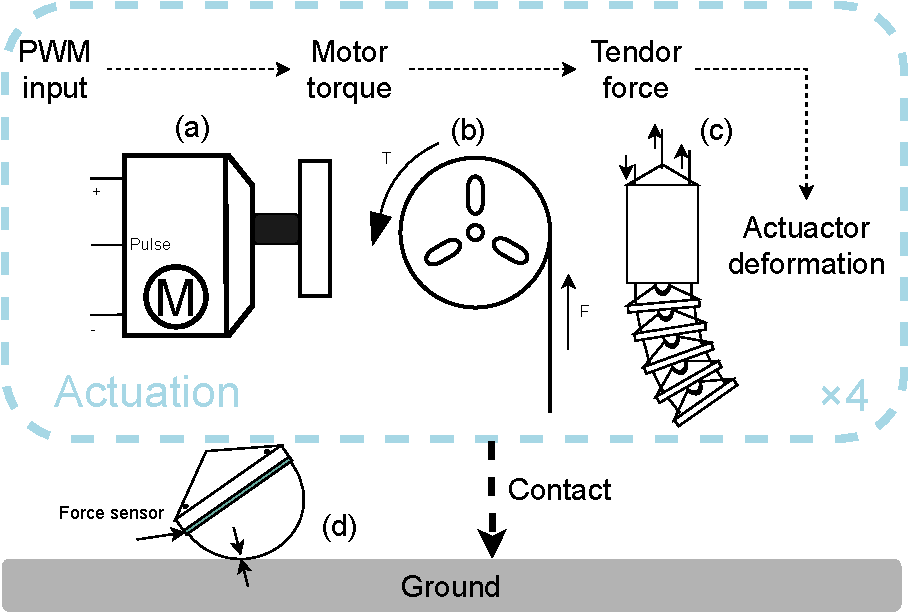
\includegraphics[width=0.9\linewidth]{img/chap3/actuation.pdf}
    \caption{Overview of the quadruped robot's main subsystems enabled by tendon-driven soft actuators. (a) Servo motor converts PWM signal to rotational motions while applying torque exerted on the rotational spool. (b) The spool translates the torque from the servo motor to the traction force in the tendon. (c) The tendon force is applied on the actuator and effectuates its deformation. (d) The actuator's deformation introduces relative motion between the robot's feet and diverse ground conditions, thereby instigating the overall locomotion of the quadruped robot. Reproduced from Ji et al.\cite{jiSynthesizingOptimalGait2022, jiOmnidirectionalWalkingQuadruped2022}}
    \label{fig:actuation}
\end{figure}
